\chapter{Keanekaragaman Hayati}\label{ch:g5:biodiversity}

Ambil satu meter persegi padang rumput yang sedang berbunga lalu
mulailah menghitung: selusin jenis \omterm{def:g1:plants-around-us:plant}{tumbuhan}, kumbang dan \omterm{prop:g3:sorting-living-things:groups}{serangga}
kecil yang tak terhitung, laba-laba, siput, cacing di bawah dan
kupu-kupu di atas. Sekarang cobalah satu meter persegi halaman sekolah
yang berpaving. Perbedaan antara kedua hitungan itu punya nama ---
\omterm{def:g5:biodiversity:biodiversity}{keanekaragaman hayati} --- dan ia telah menjadi salah satu kata
terpenting dalam \omterm{def:g1:living-or-not:living}{biologi}.

\section{Keanekaragaman kehidupan}

\begin{definition}[Spesies]\label{def:g5:biodiversity:species}
Suatu \emph{spesies}\index{spesies} adalah satu jenis \omterm{def:g1:living-or-not:living}{makhluk hidup}
tertentu: semua individu yang dibangun atas model yang sama, dan yang
berkembang biak di antara mereka sendiri. \omterm{prop:g3:sorting-living-things:groups}{Burung} pipit rumah adalah
sebuah spesies; begitu pula \omterm{def:g3:flowers-fruits-seeds:parts}{bunga} aster biasa, rubah merah, dan siput
kebun. Kelas pada \cref{ch:g4:classifying-animals} adalah kotak berisi
banyak spesies: ``\omterm{prop:g3:sorting-living-things:groups}{mamalia}'' memuat ribuan di antaranya.
\end{definition}

\begin{definition}[Keanekaragaman hayati]\label{def:g5:biodiversity:biodiversity}
Yang disebut \emph{keanekaragaman hayati}\index{keanekaragaman hayati}
sebuah tempat adalah ragam kehidupan yang dimuatnya --- terutama,
berapa banyak \emph{\omterm{def:g5:biodiversity:species}{spesies}} berbeda yang hidup di situ, dan sebaik apa
keadaan masing-masing. Padang rumput yang berbunga, yang kaya \omterm{def:g5:biodiversity:species}{spesies},
punya keanekaragaman hayati yang tinggi; halaman berpaving, hampir
tidak punya.
\end{definition}

\begin{omfigure}
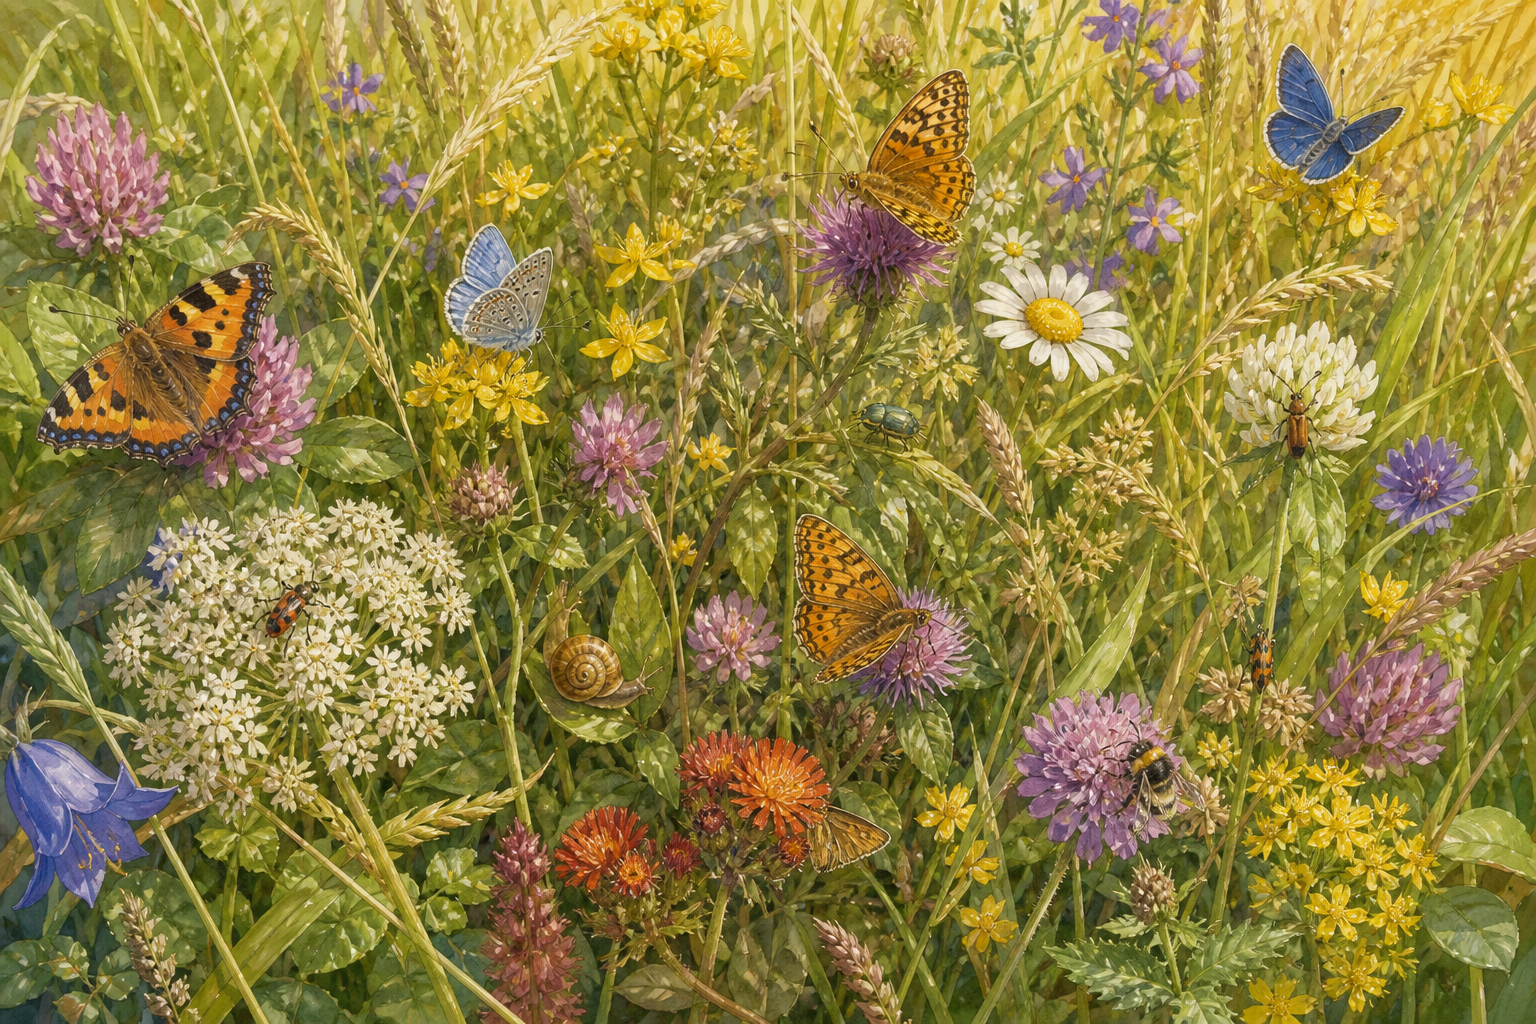
\includegraphics[width=0.62\linewidth]{images/book1/ai/g5-biodiversity-meadow.png}

{\small Satu meter persegi padang rumput, di tengah penghitungan:
rerumputan, \omterm{def:g3:flowers-fruits-seeds:parts}{bunga}, kupu-kupu, kumbang, seekor siput --- dan
penghitungannya baru saja bermula.}
\end{omfigure}

\begin{example}[Menghitung planetnya]\label{ex:g5:biodiversity:planet}
Para ilmuwan sejauh ini sudah menamai kira-kira dua juta \omterm{def:g5:biodiversity:species}{spesies} ---
dan yakin bahwa itu baru sebagian dari seluruhnya, sebab \omterm{def:g5:biodiversity:species}{spesies} baru
ditemukan pada setiap penjelajahan yang serius: terutama kumbang
(tidak ada kelompok yang punya lebih banyak \omterm{def:g5:biodiversity:species}{spesies} bernama), tetapi
juga \omterm{prop:g3:sorting-living-things:groups}{ikan}, katak, \omterm{def:g1:plants-around-us:plant}{tumbuhan}, bahkan sesekali \omterm{prop:g3:sorting-living-things:groups}{mamalia}. Jumlah \omterm{def:g5:biodiversity:species}{spesies}
Bumi yang sesungguhnya masih belum diketahui --- kebanyakan perkiraan
berjalan sampai jutaan di luar yang sudah dinamai.
\end{example}

\begin{remark}[Keanekaragaman pada setiap skala]\label{rem:g5:biodiversity:scales}
\omterm{def:g5:biodiversity:biodiversity}{Keanekaragaman hayati} terlihat pada beberapa skala sekaligus: banyak
\omterm{def:g5:biodiversity:species}{spesies} dalam satu \omterm{def:g2:where-animals-live:habitat}{habitat}; banyak \omterm{def:g2:where-animals-live:habitat}{habitat} berbeda yang berdampingan
(kolam, pagar tanaman, padang rumput --- masing-masing dengan
spesiesnya sendiri, seperti diperlihatkan
\cref{ex:g2:where-animals-live:four}); dan, di dalam satu \omterm{def:g5:biodiversity:species}{spesies},
tidak ada dua individu yang benar-benar serupa --- tidak ada dua siput
kebun yang mengenakan \omterm{def:g1:animals-around-us:covering}{cangkang} yang persis sama. Ragam di dalam ragam
di dalam ragam.
\end{remark}

\section{Mengapa keanekaragaman hayati berarti}

\begin{proposition}[Jalanya membutuhkan benangnya]\label{prop:g5:biodiversity:web}
\omterm{def:g5:biodiversity:species}{Spesies} sebuah \omterm{def:g2:where-animals-live:habitat}{habitat} saling memberi makan, melindungi, menyerbuki
dan membersihkan --- mereka adalah benang dari satu jala
(\cref{rem:g3:food-chains:web}). Jala yang kaya dan berbenang banyak
dapat menyerap guncangan: kalau satu \omterm{def:g5:biodiversity:species}{spesies} mangsa gagal, pemburunya
beralih ke \omterm{def:g5:biodiversity:species}{spesies} yang lain. Jala yang miskin mudah robek: tiap
\omterm{def:g5:biodiversity:species}{spesies} yang hilang menyisakan lebih sedikit pilihan bagi yang
selamat. \omterm{def:g5:biodiversity:biodiversity}{Keanekaragaman hayati} adalah kekuatan jalanya.
\end{proposition}
\admitted

\begin{example}[Ujian kebun buah]\label{ex:g5:biodiversity:orchard}
Sebuah kebun \omterm{prop:g3:flowers-fruits-seeds:transform}{buah} yang punya pagar tanaman, jalur \omterm{def:g3:flowers-fruits-seeds:parts}{bunga} liar dan pohon
tua menampung berlusin-lusin \omterm{def:g5:biodiversity:species}{spesies} penolong: lebah dan lalat \omterm{def:g3:flowers-fruits-seeds:parts}{bunga}
menyerbuki \omterm{def:g3:flowers-fruits-seeds:parts}{bunganya}
(\cref{rem:g3:flowers-fruits-seeds:bees}), kepik memakan kutu \omterm{def:g1:plants-around-us:parts}{daunnya},
\omterm{prop:g3:sorting-living-things:groups}{burung} berpatroli mencari \omterm{ex:g2:animals-grow-up:butterfly}{ulat}, cacing menjaga tanahnya tetap
berongga. Bongkarlah pagar tanamannya dan pangkaslah \omterm{def:g3:flowers-fruits-seeds:parts}{bunganya}, dan
para penolong itu pergi --- petani \omterm{prop:g3:flowers-fruits-seeds:transform}{buahnya} lalu harus mengerjakan
tugas mereka sendirian, tugas yang dahulu dikerjakan jalanya
cuma-cuma.
\end{example}

\begin{example}[Manusia hidup dari jalanya]\label{ex:g5:biodiversity:people}
Segala yang dimakan manusia berpangkal pada \omterm{def:g5:biodiversity:species}{spesies} yang hidup
(\cref{rem:g4:what-plants-need:everyone}); kebanyakan obat kita
pertama kali ditemukan pada \omterm{def:g1:plants-around-us:plant}{tumbuhan}, kapang dan \omterm{def:g1:living-or-not:living}{makhluk hidup} lain;
kapas, wol, kayu dan \omterm{def:g1:the-five-senses:sense}{kulit} adalah hasil \omterm{def:g5:biodiversity:species}{spesies}. Benang jalanya
melintas lurus melalui setiap dapur, apotek dan lemari pakaian.
\end{example}

\section{Keanekaragaman hayati dapat hilang --- dan dapat ditolong}

\begin{proposition}[Bagaimana keanekaragaman hilang]\label{prop:g5:biodiversity:loss}
Sebuah \omterm{def:g5:biodiversity:species}{spesies} menyusut ketika apa yang menjadi sandarannya diambil:
\begin{itemize}
  \item \emph{\omterm{def:g2:where-animals-live:habitat}{habitatnya}} dihancurkan --- kolam yang dikeringkan pada
        \cref{prop:g2:where-animals-live:loss}, pagar tanaman yang
        dibongkar, padang rumput yang dipaving;
  \item \omterm{def:g2:caring-for-nature:environment}{lingkungannya} diracuni --- sampah dan bahan kimia
        (\cref{prop:g2:caring-for-nature:harm});
  \item terlalu banyak yang diambil --- ditangkap, dipetik, atau
        diburu secara berlebihan.
\end{itemize}
Sebuah \omterm{def:g5:biodiversity:species}{spesies} yang lenyap sepenuhnya --- di mana pun, selamanya ---
disebut \emph{punah}\index{punah}. Kepunahan tidak seperti permainan
yang kalah: tidak ada babak berikutnya.
\end{proposition}
\admitted

\begin{method}[Menolong keanekaragaman hayati, mulai dari yang kecil]\label{met:g5:biodiversity:help}
Resep pada \cref{met:g2:caring-for-nature:rules} dapat diperbesar
skalanya:
\begin{enumerate}
  \item pertahankan dan tanamlah keragaman --- pagar tanaman berisi
        lima semak mengalahkan pagar kawat, jalur \omterm{def:g3:flowers-fruits-seeds:parts}{bunga} mengalahkan
        kerikil kosong;
  \item sisakan sudut yang liar: kayu mati, tumpukan \omterm{def:g1:plants-around-us:parts}{daun}, rumput yang
        tidak dipangkas adalah \omterm{def:g2:where-animals-live:habitat}{habitat}
        (\cref{ex:g2:caring-for-nature:home});
  \item tolonglah para penolong: kotak sarang, tempat berteduh
        \omterm{prop:g3:sorting-living-things:groups}{serangga}, sebuah kolam sekecil apa pun
        (\cref{ex:g2:where-animals-live:schoolpond});
  \item hitunglah apa yang hidup di sekitarmu, tahun demi tahun ---
        apa yang dihitung akan diperhatikan, dan apa yang diperhatikan
        akan dilindungi.
\end{enumerate}
\end{method}

\begin{example}[Kembalinya bangau]\label{ex:g5:biodiversity:storks}
Di tempat padang rumput basah dipulihkan dan panggung sarang
ditegakkan, bangau --- yang dahulu nyaris lenyap dari seluruh daerah
--- kembali untuk berbiak, dan bersamanya kembali pula katak, capung
serta \omterm{def:g3:flowers-fruits-seeds:parts}{bunga} padang rumput. \omterm{def:g5:biodiversity:species}{Spesies} kembali ketika benangnya diikat
ulang: perlindungan itu berhasil, dan hasilnya dapat diamati dari alun-alun
desanya.
\end{example}

\section{Latihan}

\begin{exercise}[$\star$]\label{exo:g5:biodiversity:1}
Apa itu \omterm{def:g5:biodiversity:species}{spesies}? Berikan tiga contoh dari bab ini.
\end{exercise}

\begin{exercise}[$\star$]\label{exo:g5:biodiversity:2}
Apa itu \omterm{def:g5:biodiversity:biodiversity}{keanekaragaman hayati}? Bandingkan padang rumputnya dengan
halaman berpavingnya.
\end{exercise}

\begin{exercise}[$\star$]\label{exo:g5:biodiversity:3}
Kira-kira berapa banyak \omterm{def:g5:biodiversity:species}{spesies} yang sudah dinamai sejauh ini? Mengapa
jumlah yang sesungguhnya pasti lebih tinggi?
\end{exercise}

\begin{exercise}[$\star$]\label{exo:g5:biodiversity:4}
Sebutkan ketiga skala keanekaragaman pada
\cref{rem:g5:biodiversity:scales}, masing-masing dengan contohnya.
\end{exercise}

\begin{exercise}[$\star$]\label{exo:g5:biodiversity:5}
Mengapa jala yang kaya \omterm{def:g5:biodiversity:species}{spesies} bertahan terhadap guncangan lebih baik
daripada yang miskin? Pakai alasan pemburu-beralih-mangsa.
\end{exercise}

\begin{exercise}[$\star$]\label{exo:g5:biodiversity:6}
Daftarkan empat \omterm{def:g5:biodiversity:species}{spesies} penolong di kebun \omterm{prop:g3:flowers-fruits-seeds:transform}{buahnya} dan tugas cuma-cuma
yang dikerjakan masing-masing.
\end{exercise}

\begin{exercise}[$\star$]\label{exo:g5:biodiversity:7}
Berikan tiga cara sebuah \omterm{def:g5:biodiversity:species}{spesies} menyusut, masing-masing dengan satu
contoh. Apa arti \emph{\omterm{prop:g5:biodiversity:loss}{punah}}?
\end{exercise}

\begin{exercise}[$\star$]\label{exo:g5:biodiversity:8}
Cobalah: hitunglah \omterm{def:g5:biodiversity:species}{spesies} --- \omterm{def:g1:plants-around-us:plant}{tumbuhan} dan \omterm{def:g1:animals-around-us:animal}{hewan}, yang bernama atau
yang kamu lukiskan --- di dalam satu petak kecil yang kamu pilih di
luar rumah. Lalu hitunglah satu petak berpaving sebagai pembanding.
Kedua bilanganmu adalah sebuah pengukuran \omterm{def:g5:biodiversity:biodiversity}{keanekaragaman hayati}.
\end{exercise}

\begin{exercise}[$\star\star$]\label{exo:g5:biodiversity:9}
``Kehilangan satu \omterm{def:g5:biodiversity:species}{spesies} kumbang dari ribuan tidak mungkin berarti.''
Jawablah dengan \cref{prop:g5:biodiversity:web} --- dan dengan
kenyataan bahwa tidak seorang pun mengetahui semua benang yang
dipegang sebuah \omterm{def:g5:biodiversity:species}{spesies}.
\end{exercise}

\begin{exercise}[$\star\star$]\label{exo:g5:biodiversity:10}
Kisah bangau itu disebut keberhasilan perlindungan \emph{\omterm{def:g2:where-animals-live:habitat}{habitat}}
alih-alih perlindungan bangau satu demi satu. Jelaskan perbedaannya,
dengan memakai \cref{prop:g2:where-animals-live:loss} dan apa yang
kembali bersama bangaunya.
\end{exercise}

\begin{exercise}[$\star\star\star$]\label{exo:g5:biodiversity:11}
Seorang penjaga kebun \omterm{prop:g3:flowers-fruits-seeds:transform}{buah} mengganti pagar tanaman dan jalur \omterm{def:g3:flowers-fruits-seeds:parts}{bunga}
dengan pagar kawat serta kerikil, lalu harus menyewa sarang lebah
untuk penyerbukan dan menyemprot kutu \omterm{def:g1:plants-around-us:parts}{daun} --- membelanjakan uang
untuk tugas yang dahulu dikerjakan cuma-cuma. Pakai
\cref{ex:g5:biodiversity:orchard} untuk menjelaskan apa yang
sesungguhnya disingkirkan --- dan mengapa pembukuan atas kerja
cuma-cuma alam biasanya muncul justru sesudah kerja itu berhenti.
\end{exercise}
